% ============================================================
%  MIVA-KNIGHT: Complete Technical Documentation
%  Multi-modal Industrial Voice Assistant with
%  Knowledge-Integrated Hybrid Reasoning
% ============================================================
\documentclass[12pt,a4paper]{article}

% ── Core packages ──────────────────────────────────────────
\usepackage[T1]{fontenc}
\usepackage[utf8]{inputenc}
\usepackage[margin=2.2cm]{geometry}
\usepackage{amsmath,amssymb,amsthm}
\usepackage{mathtools}
\usepackage{bm}

% ── Algorithms ─────────────────────────────────────────────
\usepackage{algorithm}
\usepackage{algpseudocode}





% ── TikZ / diagrams ────────────────────────────────────────
\usepackage{tikz}
\usetikzlibrary{
  shapes.geometric,
  shapes.multipart,
  arrows.meta,
  arrows,
  positioning,
  fit,
  calc,
  backgrounds,
  decorations.pathreplacing,
  matrix,
  shadows,
  fadings
}

% ── Colours / boxes ────────────────────────────────────────
\usepackage[dvipsnames,svgnames,table]{xcolor}
\usepackage[most]{tcolorbox}
\tcbuselibrary{theorems,skins,breakable}

% ── Tables / figures ───────────────────────────────────────
\usepackage{booktabs}
\usepackage{multirow}
\usepackage{graphicx}
\usepackage{float}
\usepackage{caption}
\usepackage{subcaption}
\usepackage{array}

% ── Typography / layout ────────────────────────────────────
%\usepackage{microtype}
\usepackage{enumitem}
\usepackage{parskip}
\usepackage{titlesec}
\usepackage{fancyhdr}
\usepackage{hyperref}
\usepackage{cleveref}

% ── Hyperref setup ─────────────────────────────────────────
\hypersetup{
  colorlinks=true,
  linkcolor=NavyBlue,
  citecolor=ForestGreen,
  urlcolor=Maroon,
  pdftitle={MIVA-KNIGHT Technical Documentation},
  pdfauthor={MIVA-KNIGHT Project}
}

% ════════════════════════════════════════════════════════════
%  COLOUR PALETTE
% ════════════════════════════════════════════════════════════
\definecolor{mivablue}{RGB}{25,84,163}
\definecolor{mivagreen}{RGB}{34,139,34}
\definecolor{mivaorange}{RGB}{210,105,30}
\definecolor{mivared}{RGB}{178,34,34}
\definecolor{mivapurple}{RGB}{106,13,173}
\definecolor{mivateal}{RGB}{0,128,128}
\definecolor{mivagray}{RGB}{100,100,100}
\definecolor{boxbg}{RGB}{245,248,255}
\definecolor{algbg}{RGB}{240,255,240}
\definecolor{warningbg}{RGB}{255,248,220}

% ════════════════════════════════════════════════════════════
%  THEOREM ENVIRONMENTS
% ════════════════════════════════════════════════════════════
\tcbset{
  mytheo/.style={
    enhanced, breakable,
    colback=boxbg, colframe=mivablue,
    fonttitle=\bfseries\color{white},
    attach boxed title to top left={yshift=-2mm,xshift=4mm},
    boxed title style={colback=mivablue, rounded corners},
    arc=3pt, outer arc=3pt,
    top=6pt, bottom=6pt
  },
  mylemma/.style={
    enhanced, breakable,
    colback=white, colframe=mivagreen,
    fonttitle=\bfseries\color{white},
    attach boxed title to top left={yshift=-2mm,xshift=4mm},
    boxed title style={colback=mivagreen, rounded corners},
    arc=3pt, outer arc=3pt
  },
  myaxiom/.style={
    enhanced, breakable,
    colback=white, colframe=mivaorange,
    fonttitle=\bfseries\color{white},
    attach boxed title to top left={yshift=-2mm,xshift=4mm},
    boxed title style={colback=mivaorange, rounded corners},
    arc=3pt, outer arc=3pt
  },
  mydef/.style={
    enhanced, breakable,
    colback=white, colframe=mivapurple,
    fonttitle=\bfseries\color{white},
    attach boxed title to top left={yshift=-2mm,xshift=4mm},
    boxed title style={colback=mivapurple, rounded corners},
    arc=3pt, outer arc=3pt
  },
  myplain/.style={
    enhanced, breakable,
    colback=warningbg, colframe=mivaorange!80,
    fonttitle=\bfseries\color{mivaorange!80!black},
    attach boxed title to top left={yshift=-2mm,xshift=4mm},
    boxed title style={colback=mivaorange!20, colframe=mivaorange!80,
                        rounded corners},
    arc=3pt, outer arc=3pt
  }
}

\newtcbtheorem[number within=section]{theorem}{Theorem}{mytheo}{thm}
\newtcbtheorem[number within=section]{lemma}{Lemma}{mylemma}{lem}
\newtcbtheorem[number within=section]{axiom}{Axiom}{myaxiom}{ax}
\newtcbtheorem[number within=section]{definition}{Definition}{mydef}{def}
\newtcbtheorem[number within=section]{proposition}{Proposition}{mytheo}{prop}

\newenvironment{plainbox}[1]{%
  \begin{tcolorbox}[myplain,title={#1}]
}{%
  \end{tcolorbox}
}

% ════════════════════════════════════════════════════════════
%  TIKZ STYLES
% ════════════════════════════════════════════════════════════
\tikzset{
  block/.style={
    rectangle, rounded corners=4pt, draw=mivablue, thick,
    fill=blue!8, minimum width=2.8cm, minimum height=0.85cm,
    text centered, font=\small\bfseries, drop shadow
  },
  blockG/.style={
    block, fill=green!10, draw=mivagreen
  },
  blockO/.style={
    block, fill=orange!10, draw=mivaorange
  },
  blockP/.style={
    block, fill=purple!10, draw=mivapurple
  },
  blockR/.style={
    block, fill=red!8, draw=mivared
  },
  blockT/.style={
    block, fill=teal!8, draw=mivateal
  },
  io/.style={
    trapezium, trapezium left angle=70, trapezium right angle=110,
    draw=mivagray, thick, fill=gray!12, minimum width=2.6cm,
    minimum height=0.75cm, text centered, font=\small\bfseries
  },
  decision/.style={
    diamond, draw=mivaorange, thick, fill=orange!10,
    minimum width=2cm, minimum height=1cm,
    text centered, font=\small\bfseries, aspect=2
  },
  arrow/.style={-{Stealth[length=7pt]}, thick, color=mivagray},
  arrowB/.style={-{Stealth[length=7pt]}, thick, color=mivablue},
  arrowG/.style={-{Stealth[length=7pt]}, thick, color=mivagreen},
  arrowR/.style={-{Stealth[length=7pt]}, thick, color=mivared},
  dasharrow/.style={-{Stealth[length=6pt]}, dashed, thick, color=mivagray!70},
  arrowT/.style={-{Stealth[length=7pt]}, thick, color=mivateal},
  groupbox/.style={
    draw=mivablue!50, dashed, thick, rounded corners=6pt,
    fill=blue!3
  }
}

% ════════════════════════════════════════════════════════════
%  HEADER / FOOTER
% ════════════════════════════════════════════════════════════
\pagestyle{fancy}
\fancyhf{}
\fancyhead[L]{\small\color{mivagray}\textbf{MIVA-KNIGHT} — Technical Documentation}
\fancyhead[R]{\small\color{mivagray}\nouppercase{\leftmark}}
\fancyfoot[C]{\small\color{mivagray}\thepage}
\renewcommand{\headrulewidth}{0.4pt}

\titleformat{\section}{\large\bfseries\color{mivablue}}{{\color{mivablue}\thesection}}{0.8em}{}[\titlerule]
\titleformat{\subsection}{\normalsize\bfseries\color{mivablue!80}}{\thesubsection}{0.6em}{}
\titleformat{\subsubsection}{\normalsize\bfseries\color{mivagray}}{\thesubsubsection}{0.5em}{}

% ════════════════════════════════════════════════════════════
%  CUSTOM COMMANDS
% ════════════════════════════════════════════════════════════
\newcommand{\kg}{\mathcal{G}}
\newcommand{\kgV}{\mathcal{V}}
\newcommand{\kgE}{\mathcal{E}}
\newcommand{\kgR}{\mathcal{R}}
\newcommand{\Enc}{\operatorname{Enc}}
\newcommand{\MHA}{\operatorname{MHA}}
\newcommand{\LN}{\operatorname{LayerNorm}}
\newcommand{\FFN}{\operatorname{FFN}}
\newcommand{\ReLU}{\operatorname{ReLU}}
\newcommand{\softmax}{\operatorname{softmax}}
\newcommand{\efused}{e_{\text{fused}}}
\newcommand{\R}{\mathbb{R}}

% ════════════════════════════════════════════════════════════
%  DOCUMENT
% ════════════════════════════════════════════════════════════
\begin{document}

% ── TITLE PAGE ─────────────────────────────────────────────
\begin{titlepage}
\begin{tikzpicture}[remember picture, overlay]
  \fill[mivablue!90] (current page.north west) rectangle
        ([yshift=-5cm]current page.north east);
  \fill[mivablue!30] (current page.south west) rectangle
        ([yshift=2cm]current page.south east);
\end{tikzpicture}

\vspace*{1.5cm}
{\centering
{\color{white}\LARGE\bfseries MIVA-KNIGHT}\\[0.4cm]
{\color{white!85!mivablue}\large
  Multi-modal Industrial Voice Assistant\\[0.2cm]
  with Knowledge-Integrated Hybrid Reasoning}\\[0.6cm]
{\color{white!70!mivablue}\normalsize Complete Technical Pipeline Documentation}\\[2cm]
}

\begin{tcolorbox}[
  enhanced, colback=white, colframe=mivablue!40,
  arc=6pt, width=0.88\textwidth, center,
  title={\textbf{Document Scope}},
  fonttitle=\bfseries\color{mivablue},
  attach boxed title to top center={yshift=-2mm},
  boxed title style={colback=white, colframe=mivablue!40}
]
This document provides a comprehensive technical and intuitive exposition of the
MIVA-KNIGHT system as implemented in the annotated Jupyter notebook
\texttt{Miva\_knight\_annotated.ipynb}. It covers:
\begin{itemize}[leftmargin=1.5em]
  \item Formal mathematical foundations (definitions, axioms, theorems, lemmas)
  \item Pseudocode algorithms for every module
  \item TikZ pipeline architecture diagrams
  \item Plain-English analogies for every concept
\end{itemize}
\end{tcolorbox}

\vfill
{\centering
\begin{tabular}{cc}
\toprule
\textbf{System} & MIVA-KNIGHT \\
\textbf{Domain} & Healthcare / Industrial AI \\
\textbf{Modalities} & Text, Image, Voice, Sensor \\
\textbf{Core Techniques} & KG, RAG, Transformer, Grad-CAM, RLHF \\
\bottomrule
\end{tabular}
}
\end{titlepage}

\tableofcontents
\clearpage

% ════════════════════════════════════════════════════════════
\section{Introduction and System Overview}
% ════════════════════════════════════════════════════════════

\subsection{What is MIVA-KNIGHT?}

MIVA-KNIGHT (\textbf{M}ulti-modal \textbf{I}ndustrial \textbf{V}oice \textbf{A}ssistant with
\textbf{K}nowledge-\textbf{N}etwork \textbf{I}ntegrated \textbf{G}raph \textbf{H}ybrid
\textbf{T}ransformer) is an end-to-end AI pipeline designed to process heterogeneous
industrial and medical data from multiple sensory channels---text, images, voice, and
numeric sensor streams---and synthesise a grounded, explainable natural language response.

\begin{plainbox}{In Plain English}
Imagine a brilliant hospital consultant who simultaneously reads the patient's medical
notes (text), studies the X-ray film (image), listens to the patient's description of
symptoms (voice), and monitors the heart-rate display (sensor)---then gives you a
clear answer \emph{and} explains exactly which piece of evidence drove that answer.
MIVA-KNIGHT is that consultant, implemented in software.
\end{plainbox}

\subsection{Design Principles}

\begin{axiom}{Modular Composition}{mod}
The MIVA-KNIGHT system is the functional composition of five independent sub-systems,
each with well-defined input/output contracts:
\[
  \text{MIVA-KNIGHT} \;=\; S_{\text{KG}} \;\circ\; S_{\text{Retrieval}}
  \;\circ\; S_{\text{Fusion}} \;\circ\; S_{\text{Reasoning}}
  \;\circ\; S_{\text{Generator}}
\]
Any sub-system may be swapped independently without altering the pipeline contract.
\end{axiom}

\begin{axiom}{Missing-Modality Robustness}{miss}
If modality $m$ is unavailable at inference time, its embedding is replaced by the
zero vector:
\[
  e_m = \mathbf{0}_{d_m} \quad \text{if modality } m \text{ is absent.}
\]
The pipeline continues without modification; the absent modality contributes zero
information but does not cause failure.
\end{axiom}

% ════════════════════════════════════════════════════════════
\section{System Architecture Pipeline}
% ════════════════════════════════════════════════════════════

\subsection{Complete Pipeline Flowchart}

The following TikZ diagram illustrates the full MIVA-KNIGHT pipeline, mirroring the
structure of the implementation notebook.

\begin{figure}[H]
\centering
\resizebox{\textwidth}{!}{%
\begin{tikzpicture}[node distance=0.55cm and 0.7cm, font=\small]

% ── INPUT ROW ──────────────────────────────────────────────
\node[io] (text_in) {Text Input};
\node[io, right=0.9cm of text_in] (img_in) {Image Input};
\node[io, right=0.9cm of img_in] (voice_in) {Voice Input};
\node[io, right=0.9cm of voice_in] (sensor_in) {Sensor Input};

% ── ENCODERS ───────────────────────────────────────────────
\node[block, below=0.7cm of text_in]   (bert)   {BERT\\Encoder};
\node[block, below=0.7cm of img_in]    (vit)    {ViT / ResNet\\Encoder};
\node[block, below=0.7cm of voice_in]  (w2v)    {Wav2Vec\\Encoder};
\node[block, below=0.7cm of sensor_in] (mlp)    {MLP\\Encoder};

% ── PROJECTION ─────────────────────────────────────────────
\node[blockG, below=0.6cm of bert]  (proj_t) {Linear Proj.\\$W_\text{text}$};
\node[blockG, below=0.6cm of vit]   (proj_i) {Linear Proj.\\$W_\text{img}$};
\node[blockG, below=0.6cm of w2v]   (proj_v) {Linear Proj.\\$W_\text{voice}$};
\node[blockG, below=0.6cm of mlp]   (proj_s) {Linear Proj.\\$W_\text{sensor}$};

% ── FUSION BOX ─────────────────────────────────────────────
\node[block, below=1.1cm of proj_i,
      minimum width=8.5cm, minimum height=1.1cm,
      xshift=0.9cm] (fusion)
  {Multi-modal Fusion Layer: Stack $[h_t;h_i;h_v;h_s]$,
   MHA (8 heads), MeanPool $\to e_\text{fused}$};

% ── KG BRANCH ──────────────────────────────────────────────
\node[blockP, left=1.8cm of fusion, yshift=-1.6cm]
  (kg) {Knowledge\\Graph $\mathcal{G}$};
\node[blockP, below=0.55cm of kg]
  (ner) {Entity\\Extraction (NER)};
\node[blockP, below=0.55cm of ner]
  (kgctx) {KG Context\\Embeddings};

% ── HYBRID RETRIEVAL ───────────────────────────────────────
\node[blockO, below=0.7cm of fusion, xshift=2.4cm]
  (dense) {Dense Retrieval\\(BERT cosine)};
\node[blockO, right=0.8cm of dense]
  (graph) {Graph Retrieval\\(LightRAG)};
\node[blockO, below=0.6cm of dense, xshift=1.2cm,
      minimum width=4.2cm]
  (hybrid) {Hybrid Score Fusion\\$\alpha\cdot s_\text{dense}+(1-\alpha)\cdot s_\text{graph}$};

% ── REASONING ──────────────────────────────────────────────
\node[block, below=2.2cm of fusion, xshift=-1.5cm,
      minimum width=6cm, minimum height=1.1cm]
  (reason) {Transformer Reasoning Module\\
            TransformerEncoder $\times 4$ + KG Cross-Attention};

% ── LOSS / TRAINING ────────────────────────────────────────
\node[blockR, left=1.2cm of reason, yshift=-1.5cm]
  (loss) {Multi-Objective\\Loss $\mathcal{L}_\text{total}$};

% ── OUTPUT ─────────────────────────────────────────────────
\node[block, below=0.65cm of reason, minimum width=5cm]
  (gen) {Response Generator\\FFN$(r)$};
\node[blockT, below=0.65cm of gen, minimum width=4cm]
  (gradcam) {Grad-CAM\\Explainability};
\node[io, below=0.65cm of gradcam, minimum width=4cm]
  (out) {Final Response\\+ Visual Explanation};

% ── ARROWS: inputs → encoders ──────────────────────────────
\draw[arrow] (text_in)   -- (bert);
\draw[arrow] (img_in)    -- (vit);
\draw[arrow] (voice_in)  -- (w2v);
\draw[arrow] (sensor_in) -- (mlp);

% ── ARROWS: encoders → projections ─────────────────────────
\draw[arrowG] (bert)  -- (proj_t);
\draw[arrowG] (vit)   -- (proj_i);
\draw[arrowG] (w2v)   -- (proj_v);
\draw[arrowG] (mlp)   -- (proj_s);

% ── ARROWS: projections → fusion ───────────────────────────
\draw[arrowB] (proj_t.south) -- ++(0,-0.3) -| (fusion.north west);
\draw[arrowB] (proj_i.south) -- ++(0,-0.3) -| ([xshift=-0.5cm]fusion.north);
\draw[arrowB] (proj_v.south) -- ++(0,-0.3) -| ([xshift=0.5cm]fusion.north);
\draw[arrowB] (proj_s.south) -- ++(0,-0.3) -| (fusion.north east);

% ── KG branch ──────────────────────────────────────────────
\draw[arrowG] (text_in.south) -- ++(0,-0.15) -- ++(-3.6,0) -- (kg.north);
\draw[arrow]  (kg) -- (ner);
\draw[arrow]  (ner) -- (kgctx);
\draw[arrowR] (kgctx.south) -- ++(0,-0.3) -| (reason.west);

% ── Fusion → retrieval ─────────────────────────────────────
\draw[arrowB] (fusion.south) -- ++(0,-0.3) -| (dense.north);
\draw[arrowB] (fusion.south) -- ++(0,-0.3) -| (graph.north);
\draw[arrow]  (dense.south)  -- (hybrid.north west);
\draw[arrow]  (graph.south)  -- (hybrid.north east);

% ── Fusion → reasoning ─────────────────────────────────────
\draw[arrowB] (fusion.south) -- ++(0,-1.4) -| (reason.north);

% ── Retrieval context → reasoning ──────────────────────────
\draw[dasharrow] (hybrid.south) -- ++(0,-0.3) -| (reason.south east);

% ── Reasoning → generator ──────────────────────────────────
\draw[arrow] (reason) -- (gen);

% ── Generator → Grad-CAM → out ─────────────────────────────
\draw[arrow] (gen)     -- (gradcam);
\draw[arrow] (gradcam) -- (out);

% ── Loss ───────────────────────────────────────────────────
\draw[arrowR,dashed] (reason.west) -- (loss.north);
\draw[arrowR,dashed] (gen.west) -- ++(−0.3,0) |- (loss.east);

% ── Background groups ──────────────────────────────────────
\begin{scope}[on background layer]
  \node[groupbox, fit=(bert)(vit)(w2v)(mlp)(proj_t)(proj_i)(proj_v)(proj_s),
        label={[mivablue!70, font=\footnotesize\bfseries]above:Modality Encoders}]
        (enc_group) {};
  \node[groupbox, draw=mivagreen!60, fill=green!3,
        fit=(fusion),
        label={[mivagreen!80, font=\footnotesize\bfseries]above:Fusion Layer}]
        {};
  \node[groupbox, draw=mivaorange!60, fill=orange!3,
        fit=(dense)(graph)(hybrid),
        label={[mivaorange!80, font=\footnotesize\bfseries]right:Hybrid Retrieval}]
        {};
  \node[groupbox, draw=mivapurple!60, fill=purple!3,
        fit=(kg)(ner)(kgctx),
        label={[mivapurple!80, font=\footnotesize\bfseries]left:KG Module}]
        {};
  \node[groupbox, fit=(reason)(gen),
        label={[mivablue!70, font=\footnotesize\bfseries]above:Reasoning \& Generation}]
        {};
\end{scope}

\end{tikzpicture}
}
\caption{MIVA-KNIGHT end-to-end pipeline architecture. Arrows show data flow; dashed arrows show training signal (loss).}
\label{fig:pipeline}
\end{figure}

% ════════════════════════════════════════════════════════════
\section{Knowledge Graph Integration}
% ════════════════════════════════════════════════════════════

\subsection{Formal Definition}

\begin{definition}{Knowledge Graph}{kg}
A \emph{Knowledge Graph} is a directed, typed multigraph:
\[
  \kg \;=\; (\kgV,\;\kgE,\;\kgR)
\]
where:
\begin{itemize}
  \item $\kgV$ is the set of \textbf{entity nodes} (e.g.\ \texttt{liver}, \texttt{tumor})
  \item $\kgE \subseteq \kgV \times \kgR \times \kgV$ is the set of \textbf{typed edges}
        (relation triples $(h, r, t)$)
  \item $\kgR$ is the set of \textbf{relation types}
        (e.g.\ \texttt{contains}, \texttt{indicates}, \texttt{symptom\_of})
\end{itemize}
Each triple $(h, r, t)$ reads: ``head entity $h$ is related to tail entity $t$ by
relation $r$.''
\end{definition}

\begin{definition}{$k$-Hop Neighbourhood}{khop}
The $k$-hop neighbourhood $\mathcal{N}_k(v)$ of node $v$ is the set of all nodes
reachable from $v$ in at most $k$ traversal steps:
\[
  \mathcal{N}_k(v) = \bigcup_{i=1}^{k}
    \bigl\{\,u \in \kgV \mid \exists \text{ path of length } i
    \text{ from } v \text{ to } u\,\bigr\}
\]
\end{definition}

\subsection{DFS Multi-Hop Traversal}

\begin{theorem}{Completeness of DFS Traversal}{dfs}
The recursive DFS algorithm \textup{(Algorithm~\ref{alg:dfs})} visiting both forward
and inverse edges visits every node in $\mathcal{N}_k(v)$ exactly once, provided the
\emph{visited} set prevents re-entry.
\end{theorem}

\begin{algorithm}[H]
\caption{Multi-Hop DFS Neighbourhood Traversal}
\label{alg:dfs}
\begin{algorithmic}[1]
\Require entity identifier $v$, depth limit $k$
\Ensure $\textit{neighbors}$: list of tuples $(h, r, t, \text{depth})$
\State $\textit{visited} \leftarrow \emptyset$
\State $\textit{neighbors} \leftarrow [\,]$
\Procedure{DFS}{$\textit{current},\, \textit{hops}$}
  \If{$\textit{hops} > k$ \textbf{or} $\textit{current} \in \textit{visited}$}
    \Return
  \EndIf
  \State $\textit{visited} \leftarrow \textit{visited} \cup \{\textit{current}\}$
  \ForAll{$(h, r, t) \in \kgE$}
    \If{$h = \textit{current}$ \textbf{and} $t \notin \textit{visited}$}
      \State $\textit{neighbors}.\text{append}(h, r, t, \textit{hops})$  \Comment{Forward edge} \State \Call{DFS}{$t,\; \textit{hops}+1$}
    \ElsIf{$t = \textit{current}$ \textbf{and} $h \notin \textit{visited}$}
      \State $\textit{neighbors}.\text{append}(t, r^{-1}, h, \textit{hops})$  \Comment{Inverse edge} \State \Call{DFS}{$h,\; \textit{hops}+1$}
    \EndIf
  \EndFor
\EndProcedure
\State \textbf{call} \Call{DFS}{$v,\; 1$}
\State \Return $\textit{neighbors}$
\end{algorithmic}
\end{algorithm}

\begin{algorithm}[H]
\caption{DFS Path Finding Between Two KG Nodes}
\label{alg:path}
\begin{algorithmic}[1]
\Require start node $s$, target node $t$, max hops $k$
\Ensure $\textit{paths}$: list of all simple paths $s \rightsquigarrow t$
\State $\textit{paths} \leftarrow [\,]$
\Procedure{DFSPath}{$\textit{current},\; \textit{target},\; \textit{path},\; \textit{hops}$}
  \If{$\textit{hops} > k$} \Return \EndIf
  \If{$\textit{current} = \textit{target}$}
    \State $\textit{paths}.\text{append}(\text{copy}(\textit{path}))$
    \Return
  \EndIf
  \ForAll{$(h, r, t') \in \kgE$}
    \If{$h = \textit{current}$ \textbf{and}
        $t' \notin \{p[0] : p \in \textit{path}\}$}
      \State $\textit{path}.\text{push}((t', r, \textit{hops}))$ \State \Call{DFSPath}{$t',\;\textit{target},\;\textit{path},\;\textit{hops}+1$}
      \State $\textit{path}.\text{pop}()$ \Comment{Backtrack}
    \EndIf
  \EndFor
\EndProcedure
\State \textbf{call} \Call{DFSPath}{$s,\; t,\; [],\; 1$}
\State \Return $\textit{paths}$
\end{algorithmic}
\end{algorithm}

\subsection{Healthcare Knowledge Graph Diagram}

\begin{figure}[H]
\centering
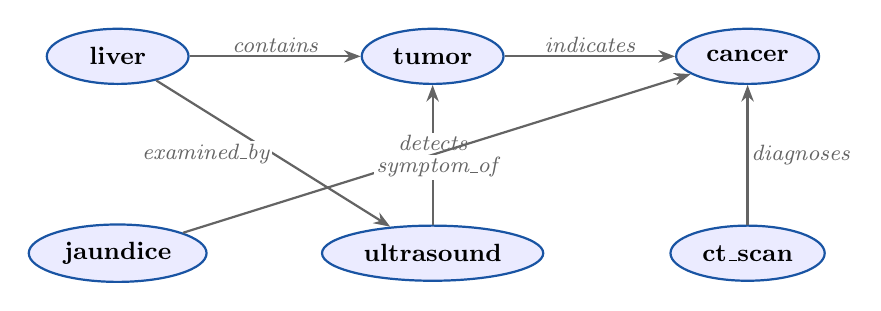
\begin{tikzpicture}[
  entity/.style={ellipse, draw=mivablue, thick, fill=blue!8,
                 minimum width=1.8cm, minimum height=0.7cm,
                 font=\small\bfseries},
  rel/.style={-{Stealth[length=6pt]}, thick, mivagray},
  rlabel/.style={font=\footnotesize\itshape, mivagray,
                 fill=white, inner sep=1pt}
]
\node[entity] (liver)      at (0,0)     {liver};
\node[entity] (tumor)      at (4,0)     {tumor};
\node[entity] (cancer)     at (8,0)     {cancer};
\node[entity] (us)         at (4,-2.5)  {ultrasound};
\node[entity] (ct)         at (8,-2.5)  {ct\_scan};
\node[entity] (jaundice)   at (0,-2.5)  {jaundice};

\draw[rel] (liver)    -- node[rlabel,above]{contains}   (tumor);
\draw[rel] (tumor)    -- node[rlabel,above]{indicates}  (cancer);
\draw[rel] (liver)    -- node[rlabel,left]{examined\_by}(us);
\draw[rel] (us)       -- node[rlabel,above]{detects}    (tumor);
\draw[rel] (ct)       -- node[rlabel,right]{diagnoses}  (cancer);
\draw[rel] (jaundice) -- node[rlabel,below]{symptom\_of}(cancer);
\end{tikzpicture}
\caption{Sample healthcare Knowledge Graph used in MIVA-KNIGHT. Nodes are entities; directed labelled edges are relation triples.}
\label{fig:kg}
\end{figure}

\begin{plainbox}{In Plain English}
Think of the Knowledge Graph as a very precise mind-map. Each bubble is a medical
concept (\emph{liver}, \emph{tumor}, \emph{jaundice}) and each arrow is a labelled
relationship (\emph{``liver \textbf{contains} tumor''}).
The DFS algorithm is like a maze-walker who explores outwards from your starting point,
remembers every corridor visited, and records everything found within $k$ steps.
The path-finder asks: ``How can I get from \emph{liver} to \emph{cancer}?'' and
traces every possible route, backtracking when it hits a dead-end.
\end{plainbox}

% ════════════════════════════════════════════════════════════
\section{Hybrid Retrieval Mechanism (RAG-LightRAG)}
% ════════════════════════════════════════════════════════════

\subsection{Dense Retrieval}

\begin{definition}{BERT Mean-Pool Encoding}{enc}
Given an input text $x$, the encoder produces:
\[
  \Enc(x) = \frac{1}{T}\sum_{t=1}^{T} h_t^{(L)}
  \;\in\; \R^{d_{\text{model}}}
\]
where $h_t^{(L)}$ is the hidden state of token $t$ at BERT's final layer $L$,
and $T$ is the sequence length.
\end{definition}

\begin{definition}{Cosine Similarity Score}{cos}
\[
  \text{score}_{\text{dense}}(q, d)
  = \cos\!\bigl(\Enc(q),\,\Enc(d)\bigr)
  = \frac{\Enc(q)\cdot\Enc(d)}{\|\Enc(q)\|\;\|\Enc(d)\|}
  \;\in\; [-1, 1]
\]
\end{definition}

\begin{lemma}{Cosine Symmetry}{cosym}
$\text{score}_{\text{dense}}(q,d) = \text{score}_{\text{dense}}(d,q)$
for all $q, d$ with non-zero norms. Proof: follows directly from the commutativity
of the dot product.
\end{lemma}

\subsection{Graph-Based Retrieval}

\begin{definition}{Path Weight}{pw}
For a path $p$ of length $|p|$, the path weight is:
\[
  w(p) = \frac{1}{|p|+1}
\]
Shorter paths receive higher weight---they represent more direct connections.
\end{definition}

\begin{definition}{Graph Retrieval Score}{grs}
\[
  \text{score}_{\text{graph}}(q, e)
  = \sum_{p \in \mathcal{P}(q, e)} w(p) \cdot \text{rel}(p)
\]
where $\mathcal{P}(q,e)$ is the set of KG paths from a query-entity to $e$,
and $\text{rel}(p)$ is a heuristic relevance score for path $p$.
\end{definition}

\subsection{Hybrid Score Combination}

\begin{theorem}{Hybrid Score Completeness}{hybrid}
Let $\alpha \in [0,1]$. The hybrid score
\[
  \boxed{\text{score}_{\text{hybrid}}(q, c)
  = \alpha \cdot \text{score}_{\text{dense}}(q, c)
  + (1-\alpha) \cdot \text{score}_{\text{graph}}(q, c)}
\]
satisfies: (i) it degenerates to pure dense retrieval when $\alpha=1$;
(ii) it degenerates to pure graph retrieval when $\alpha=0$;
(iii) it is a convex combination, so the score range is bounded by the
ranges of its components.
\end{theorem}

\begin{algorithm}[H]
\caption{Hybrid Retrieval Pipeline}
\label{alg:hybrid}
\begin{algorithmic}[1]
\Require query $q$, document corpus $\mathcal{D}$, mixing weight $\alpha$, top-$k$
\Ensure ranked list of $(c,\, \text{score})$ pairs
\State \textbf{--- Step 1: Dense Retrieval ---}
\State $\hat{q} \leftarrow \Enc(q)$
\For{each $d_i \in \mathcal{D}$}
  \State $s_{\text{dense}}[d_i] \leftarrow \cos(\hat{q},\, \Enc(d_i))$
\EndFor
\State $\mathcal{R}_{\text{dense}} \leftarrow \text{top-}k(s_{\text{dense}})$
\State
\State \textbf{--- Step 2: Graph Retrieval ---}
\State $\mathcal{E}_q \leftarrow \text{extract\_entities}(q)$
\State $\mathcal{R}_{\text{graph}} \leftarrow [\,]$
\For{each entity $e \in \mathcal{E}_q$}
  \State $N \leftarrow \text{KG.get\_neighbors}(e, k=2)$
  \For{each neighbour $n \in N$}
    \State $\mathcal{R}_{\text{graph}}.\text{append} \bigl(n,\; w(p) \cdot \text{rel}(p)\bigr)$
  \EndFor
\EndFor
\State
\State \textbf{--- Step 3: Score Fusion ---}
\State $C \leftarrow \{\}$
\For{$(d, s) \in \mathcal{R}_{\text{dense}}$}
  \State $C[d] \mathrel{+}= \alpha \cdot s$
\EndFor
\For{$(d, s) \in \mathcal{R}_{\text{graph}}$}
  \State $C[d] \mathrel{+}= (1-\alpha) \cdot s$
\EndFor
\State \Return $\text{sort}(C, \text{descending})[:k]$
\end{algorithmic}
\end{algorithm}

\begin{figure}[H]
\centering
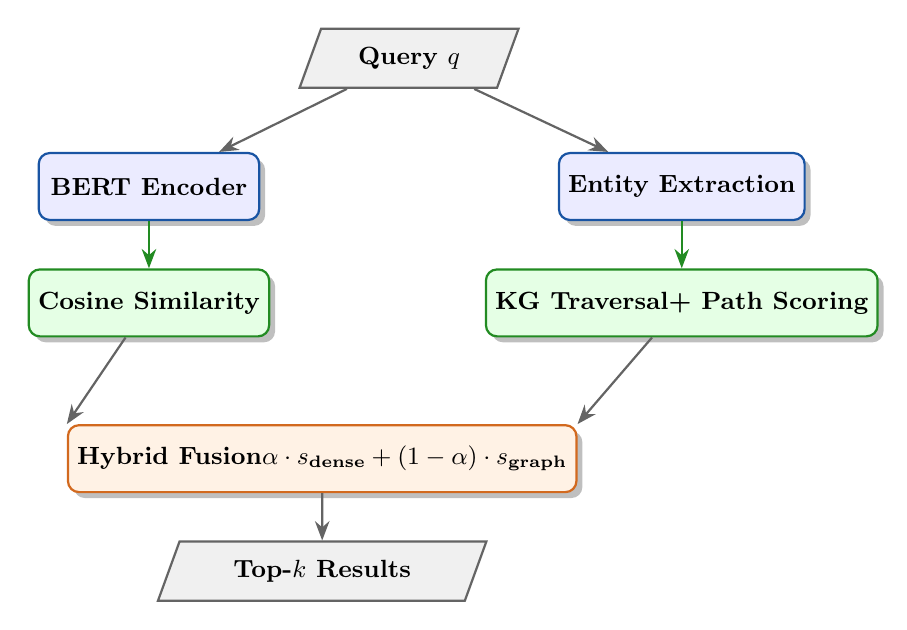
\begin{tikzpicture}[node distance=0.65cm and 1.0cm]
  \node[io] (q) {Query $q$};
  \node[block, below left=0.8cm and 1.5cm of q]  (bert2) {BERT Encoder};
  \node[block, below right=0.8cm and 1.5cm of q] (ner2)  {Entity Extraction};
  \node[blockG, below=0.6cm of bert2]  (cos2)  {Cosine Similarity};
  \node[blockG, below=0.6cm of ner2]   (kgtr)  {KG Traversal\\+ Path Scoring};
  \node[blockO, below=1.1cm of cos2, xshift=2.2cm,
        minimum width=4.5cm]           (fuse2) {Hybrid Fusion\\
        $\alpha \cdot s_\text{dense} + (1-\alpha)\cdot s_\text{graph}$};
  \node[io,    below=0.6cm of fuse2]   (topk)  {Top-$k$ Results};

  \draw[arrow]  (q) -- (bert2);
  \draw[arrow]  (q) -- (ner2);
  \draw[arrowG] (bert2) -- (cos2);
  \draw[arrowG] (ner2)  -- (kgtr);
  \draw[arrow]  (cos2)  -- (fuse2.north west);
  \draw[arrow]  (kgtr)  -- (fuse2.north east);
  \draw[arrow]  (fuse2) -- (topk);
\end{tikzpicture}
\caption{Hybrid retrieval flowchart. Left branch: BERT-based dense retrieval.
Right branch: KG path-based graph retrieval. Both streams merge at the fusion node.}
\label{fig:retrieval}
\end{figure}

\begin{plainbox}{In Plain English}
Imagine searching for a medical document.
\begin{itemize}
  \item \textbf{Dense retrieval} is like Google: it understands meaning and returns
        semantically similar documents.
  \item \textbf{Graph retrieval} is like a specialist's reference index: it follows
        chains of medical facts (\emph{liver} $\to$ \emph{tumor} $\to$
        \emph{cancer}).
  \item \textbf{Hybrid fusion} votes: trust Google 60\,\% and the specialist 40\,\%
        ($\alpha=0.6$), then pick the top results. This beats either method alone.
\end{itemize}
\end{plainbox}

% ════════════════════════════════════════════════════════════
\section{Multi-Modal Fusion Layer}
% ════════════════════════════════════════════════════════════

\subsection{Motivation and Projection}

Each modality has a different embedding dimension. A linear projection maps
every modality into a shared $d$-dimensional space:

\begin{definition}{Modality Projection}{modproj}
For modality $m \in \{\text{text, image, voice, sensor}\}$:
\[
  h_m = W_m \cdot e_m + b_m \;\in\; \R^{d}, \qquad d = 512
\]
where $W_m \in \R^{d \times d_m}$ and $b_m \in \R^d$ are learned parameters.
\end{definition}

\begin{table}[H]
\centering
\caption{Modality dimensions before and after projection.}
\begin{tabular}{lccc}
\toprule
\textbf{Modality} & \textbf{Encoder} & \textbf{Raw dim $d_m$} & \textbf{Projected dim} \\
\midrule
Text   & BERT        & 768  & 512 \\
Image  & ResNet/ViT  & 2048 & 512 \\
Voice  & Wav2Vec     & 512  & 512 \\
Sensor & MLP         & 256  & 512 \\
\bottomrule
\end{tabular}
\end{table}

\subsection{Multi-Head Self-Attention}

\begin{definition}{Scaled Dot-Product Attention}{sdpa}
For query matrix $Q$, key matrix $K$, value matrix $V \in \R^{n \times d_k}$:
\[
  \text{Attention}(Q, K, V)
  = \softmax\!\left(\frac{QK^\top}{\sqrt{d_k}}\right) V
\]
\end{definition}

\begin{definition}{Multi-Head Attention (MHA)}{mha}
\[
  \MHA(\mathbf{X}) = \text{Concat}(\text{head}_1,\ldots,\text{head}_H)\,W^O
\]
where $\text{head}_i = \text{Attention}(\mathbf{X}W_i^Q,\;\mathbf{X}W_i^K,\;\mathbf{X}W_i^V)$.
The self-attention uses $\mathbf{X}$ as query, key, and value simultaneously,
allowing each modality to attend to every other modality.
\end{definition}

\subsection{Residual Connections and Layer Normalisation}

\begin{definition}{Transformer Fusion Block}{tfblock}
Given stacked modality embeddings
$\mathbf{X} = [h_\text{text};\,h_\text{image};\,h_\text{voice};\,h_\text{sensor}]
\in \R^{4 \times d}$:
\begin{align}
  \mathbf{X}' &= \LN\!\bigl(\mathbf{X} + \MHA(\mathbf{X})\bigr) \label{eq:res1}\\
  \mathbf{X}''&= \LN\!\bigl(\mathbf{X}' + \FFN(\mathbf{X}')\bigr) \label{eq:res2}\\
  \efused     &= \frac{1}{4}\sum_{m=1}^{4} x''_m \;\in\; \R^d \label{eq:pool}
\end{align}
where $\FFN(x) = W_2\,\ReLU(W_1 x + b_1) + b_2$ with hidden dim $4d$.
\end{definition}

\begin{lemma}{Residual Gradient Flow}{resgrad}
With residual connections as in \eqref{eq:res1}--\eqref{eq:res2}, the gradient with
respect to the input satisfies:
\[
  \frac{\partial \mathcal{L}}{\partial \mathbf{X}}
  = \frac{\partial \mathcal{L}}{\partial \mathbf{X}'}
    \cdot \left(I + \frac{\partial\, \MHA(\mathbf{X})}{\partial \mathbf{X}}\right)
\]
The identity matrix $I$ ensures a gradient of at least $1$ flows back through each
block, preventing the \emph{vanishing gradient} problem.
\end{lemma}

\begin{algorithm}[H]
\caption{Multi-Modal Fusion Forward Pass}
\label{alg:fusion}
\begin{algorithmic}[1]
\Require modality embeddings $e_\text{text}\in\R^{768}$, $e_\text{img}\in\R^{2048}$, $e_\text{voice}\in\R^{512}$, $e_\text{sensor}\in\R^{256}$
\Ensure $\efused \in \R^{512}$, attention weights $A \in \R^{H \times 4 \times 4}$
\State $h_m \leftarrow W_m e_m + b_m$ for $m \in \{t, i, v, s\}$  \Comment{Project to $\R^{512}$}
\State $\mathbf{X} \leftarrow [h_t;\,h_i;\,h_v;\,h_s]$  \Comment{Stack: shape $[4, 512]$}
\State $\mathbf{X} \leftarrow \LN(\mathbf{X})$
\State $\mathbf{X}_\text{attn}, A \leftarrow \MHA(\mathbf{X}, \mathbf{X}, \mathbf{X})$
  \Comment{Self-attention}
\State $\mathbf{X} \leftarrow \LN(\mathbf{X} + \mathbf{X}_\text{attn})$  \Comment{Residual + LayerNorm}
\State $\mathbf{X} \leftarrow \LN(\mathbf{X} + \FFN(\mathbf{X}))$  \Comment{FFN + residual}
\State $\efused \leftarrow \frac{1}{4}\sum_{m=1}^{4} \mathbf{X}[m]$  \Comment{Mean pool over 4 modalities}
\State $\efused \leftarrow W_O\,\efused + b_O$  \Comment{Output projection}
\State \Return $\efused,\; A$
\end{algorithmic}
\end{algorithm}

\begin{figure}[H]
\centering
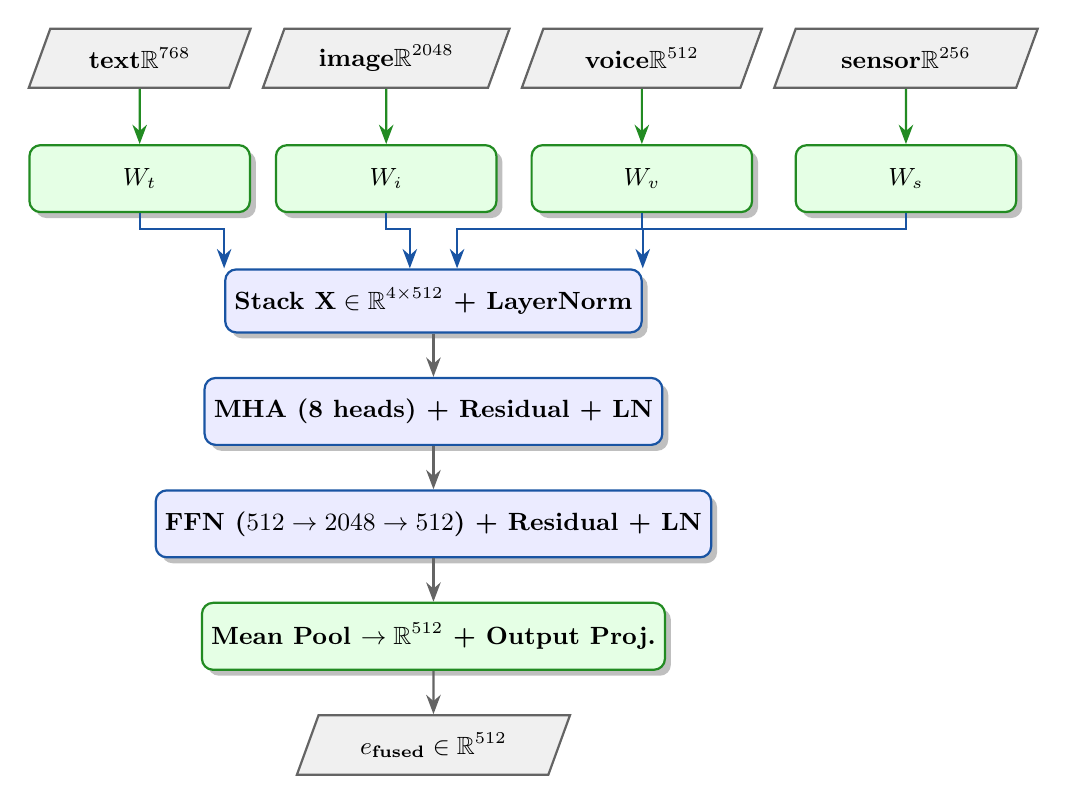
\begin{tikzpicture}[node distance=0.6cm and 0.5cm, font=\small]
  \node[io] (t) {text\\$\R^{768}$};
  \node[io, right=0.4cm of t]  (i) {image\\$\R^{2048}$};
  \node[io, right=0.4cm of i]  (v) {voice\\$\R^{512}$};
  \node[io, right=0.4cm of v]  (s) {sensor\\$\R^{256}$};

  \node[blockG, below=0.7cm of t]  (pt) {$W_t$};
  \node[blockG, below=0.7cm of i]  (pi) {$W_i$};
  \node[blockG, below=0.7cm of v]  (pv) {$W_v$};
  \node[blockG, below=0.7cm of s]  (ps) {$W_s$};

  \node[block, below=0.7cm of pi, xshift=0.6cm,
        minimum width=5.0cm, minimum height=0.8cm]
    (stack) {Stack $\mathbf{X} \in \R^{4\times 512}$ + LayerNorm};

  \node[block, below=0.55cm of stack, minimum width=5.0cm]
    (mha2) {MHA (8 heads) + Residual + LN};

  \node[block, below=0.55cm of mha2, minimum width=5.0cm]
    (ffn2) {FFN ($512 \to 2048 \to 512$) + Residual + LN};

  \node[blockG, below=0.55cm of ffn2, minimum width=5.0cm]
    (pool) {Mean Pool $\to \R^{512}$ + Output Proj.};

  \node[io, below=0.55cm of pool, minimum width=3.5cm]
    (ef) {$e_\text{fused} \in \R^{512}$};

  \foreach \x in {t,i,v,s}
    \draw[arrowG] (\x) -- (p\x);

  \draw[arrowB] (pt.south) -- ++(0,-0.2) -| (stack.north west);
  \draw[arrowB] (pi.south) -- ++(0,-0.2) -| ([xshift=-0.3cm]stack.north);
  \draw[arrowB] (pv.south) -- ++(0,-0.2) -| ([xshift=0.3cm]stack.north);
  \draw[arrowB] (ps.south) -- ++(0,-0.2) -| (stack.north east);

  \draw[arrow] (stack) -- (mha2);
  \draw[arrow] (mha2) -- (ffn2);
  \draw[arrow] (ffn2) -- (pool);
  \draw[arrow] (pool) -- (ef);
\end{tikzpicture}
\caption{Multi-modal fusion layer architecture.}
\label{fig:fusion}
\end{figure}

\begin{plainbox}{In Plain English}
Imagine the four modalities as four people speaking different languages. The projection
step is like hiring a translator who converts everyone into the same language (a
512-dimensional vector space). The self-attention step lets everyone
\emph{read each other's translated summaries} and decide whose information is most
useful for this particular question. The residual connections act as a ``memory
backup'': even if attention changes things a lot, the original information is never
completely forgotten. Mean pooling collapses the four summaries into one final briefing
document, which is passed to the reasoning module.
\end{plainbox}

% ════════════════════════════════════════════════════════════
\section{Contrastive Learning for Cross-Modal Alignment}
% ════════════════════════════════════════════════════════════

\subsection{InfoNCE Loss}

\begin{definition}{InfoNCE (Noise-Contrastive Estimation) Loss}{infonce}
For a batch of $N$ matched pairs $(e_i^{(1)}, e_i^{(2)})$ from two modalities:
\[
  \mathcal{L}_{\text{InfoNCE}}
  = -\sum_{i=1}^{N} \log
    \frac{\exp\!\bigl(\text{sim}(e_i^{(1)},\;e_i^{(2)})/\tau\bigr)}
         {\sum_{k=1}^{N}\exp\!\bigl(\text{sim}(e_i^{(1)},\;e_k^{(2)})/\tau\bigr)}
\]
where $\tau > 0$ is a \emph{temperature} hyperparameter.
\end{definition}

\begin{definition}{$N\times N$ Similarity Matrix}{simmat}
Normalise embeddings: $\hat{e} = e/\|e\|_2$.
Then construct:
\[
  S_{ij} = \frac{\hat{e}_i^{(1)} \cdot \hat{e}_j^{(2)}}{\tau},
  \quad i,j \in \{1,\ldots,N\}
\]
The InfoNCE loss is equivalent to cross-entropy with labels $y = [1, 2, \ldots, N]$
(i.e.\ each row should classify to its diagonal column):
\[
  \mathcal{L} = \text{CrossEntropy}(S,\; \mathbf{I}_N)
\]
\end{definition}

\begin{lemma}{Temperature Effect on Loss Gradient}{tempgrad}
The gradient of $\mathcal{L}_{\text{InfoNCE}}$ with respect to positive-pair
similarity $S_{ii}$ satisfies $\|\nabla_{S_{ii}}\mathcal{L}\| \propto 1/\tau$.
As $\tau \to 0$, gradients become very large (hard learning); as $\tau \to \infty$,
gradients vanish. The empirically optimal range is $\tau \in [0.05, 0.2]$.
MIVA-KNIGHT uses $\tau = 0.07$.
\end{lemma}

\begin{algorithm}[H]
\caption{Contrastive Loss (InfoNCE)}
\label{alg:contrastive}
\begin{algorithmic}[1]
\Require embeddings $E_1, E_2 \in \R^{N \times d}$ from two modalities; temperature $\tau$
\Ensure scalar loss $\mathcal{L}$
\State $\hat{E}_1 \leftarrow E_1 / \|E_1\|_2$  \Comment{L2-normalise rows}
\State $\hat{E}_2 \leftarrow E_2 / \|E_2\|_2$
\State $S \leftarrow \hat{E}_1\,\hat{E}_2^\top / \tau$  \Comment{$N\times N$ similarity matrix}
\State $y \leftarrow [0,\,1,\,2,\,\ldots,\,N-1]$  \Comment{Diagonal = positive pairs}
\State $\mathcal{L} \leftarrow \text{CrossEntropy}(S,\; y)$
\State \Return $\mathcal{L}$
\end{algorithmic}
\end{algorithm}

\begin{figure}[H]
\centering
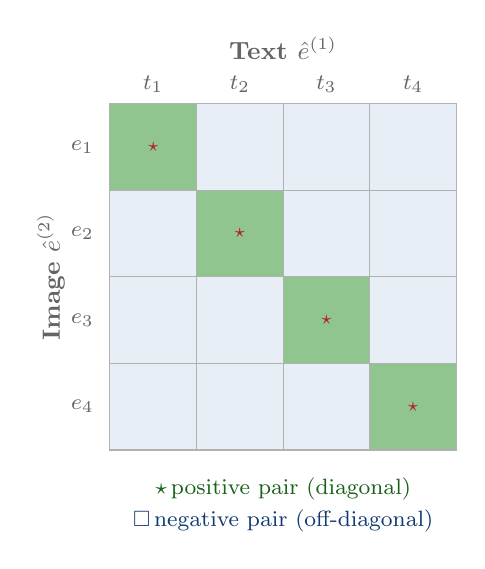
\begin{tikzpicture}[font=\small]
  % Grid
  \def\n{4}
  \foreach \i in {1,...,\n} {
    \foreach \j in {1,...,\n} {
      \pgfmathsetmacro{\isdiag}{(\i==\j)?1:0}
      \ifnum\i=\j
        \fill[mivagreen!50] ({(\j-1)*1.1},{(\n-\i)*1.1}) rectangle
             ({(\j)*1.1},{(\n-\i+1)*1.1});
      \else
        \fill[mivablue!10] ({(\j-1)*1.1},{(\n-\i)*1.1}) rectangle
             ({(\j)*1.1},{(\n-\i+1)*1.1});
      \fi
      \draw[mivagray!50] ({(\j-1)*1.1},{(\n-\i)*1.1}) rectangle
           ({(\j)*1.1},{(\n-\i+1)*1.1});
    }
  }
  % Labels on axes
  \foreach \i/\lbl in {1/$e_4$,2/$e_3$,3/$e_2$,4/$e_1$} {
    \node[font=\footnotesize,mivagray] at (-0.35,{(\i-0.5)*1.1}) {\lbl};
  }
  \foreach \j/\lbl in {1/$t_1$,2/$t_2$,3/$t_3$,4/$t_4$} {
    \node[font=\footnotesize,mivagray] at ({(\j-0.5)*1.1},4.65) {\lbl};
  }
  % Star markers on diagonal
  \foreach \i in {1,...,\n} {
    \node[font=\bfseries\scriptsize, mivared] at
         ({(\i-0.5)*1.1},{(\n-\i+0.5)*1.1}) {$\star$};
  }
  % Legend
  \node[font=\footnotesize] at (2.2,-0.5)
    {\color{mivagreen!70!black}$\star$\,positive pair (diagonal)};
  \node[font=\footnotesize] at (2.2,-0.9)
    {\color{mivablue!70!black}$\square$\,negative pair (off-diagonal)};
  % Axes labels
  \node[rotate=90,font=\small\bfseries,mivagray] at (-0.75,2.2)
    {Image $\hat{e}^{(2)}$};
  \node[font=\small\bfseries,mivagray] at (2.2,5.1)
    {Text $\hat{e}^{(1)}$};
\end{tikzpicture}
\caption{$4\times4$ similarity matrix for a batch of size 4. Green diagonal cells
are positive pairs. The loss drives diagonal scores high and off-diagonal scores low.}
\label{fig:simmat}
\end{figure}

\begin{plainbox}{In Plain English}
Imagine a classroom game: you have four text descriptions and four images that match
them (like a matching exercise). The model must pair each text with its correct image
in a lineup of all four. If it picks the wrong one, it gets penalised.
Temperature $\tau$ controls the strictness of the marking: a very small $\tau$ means
you only score full marks if you were very confident and correct. Over many batches,
the model learns that ``liver tumour text'' and ``liver tumour scan'' should be
neighbours in the embedding space.
\end{plainbox}

% ════════════════════════════════════════════════════════════
\section{Transformer Reasoning Module}
% ════════════════════════════════════════════════════════════

\subsection{Architecture}

\begin{definition}{Transformer Encoder Layer}{telayer}
A single Transformer encoder layer applies two sub-layers with residual connections:
\begin{align}
  \mathbf{z}^{(\ell)} &=
    \LN\!\bigl(\mathbf{z}^{(\ell-1)} + \MHA(\mathbf{z}^{(\ell-1)})\bigr)
    \label{eq:enc1} \\
  \mathbf{z}^{(\ell)} &\leftarrow
    \LN\!\bigl(\mathbf{z}^{(\ell)} + \FFN(\mathbf{z}^{(\ell)})\bigr)
    \label{eq:enc2}
\end{align}
The module stacks $L=4$ such layers.
\end{definition}

\begin{definition}{Learned Positional Encoding}{lpe}
The model uses a trainable positional embedding:
\[
  x' = x + \text{PE}[:\!1\!:],
  \quad \text{PE} \in \R^{1 \times T_{\max} \times d}
\]
This shifts embeddings to encode sequential position without fixing a sinusoidal
pattern, allowing the model to adapt to different sequence lengths.
\end{definition}

\subsection{Knowledge Graph Cross-Attention}

\begin{definition}{KG Cross-Attention}{kgcross}
After transformer encoding, the hidden state $x \in \R^{1 \times d}$ attends
over KG entity embeddings $\mathbf{K}_{\text{KG}} \in \R^{n_e \times d}$:
\[
  x_{\text{KG}} = \text{Attention}(
    \underbrace{x}_{\text{Query}},\;
    \underbrace{\mathbf{K}_{\text{KG}}}_{\text{Keys}},\;
    \underbrace{\mathbf{K}_{\text{KG}}}_{\text{Values}})
\]
\[
  x_{\text{final}} = x + x_{\text{KG}} \quad (\text{residual})
\]
This is a \emph{cross-attention} step: the query comes from the model's hidden state,
while keys and values come from the knowledge graph.
\end{definition}

\begin{theorem}{KG Cross-Attention Grounding}{kgground}
By computing $x_{\text{KG}}$ as the KG-attended update, the output satisfies:
\[
  x_{\text{final}} = x + \softmax\!\left(\frac{x\,\mathbf{K}_{\text{KG}}^\top}
  {\sqrt{d_k}}\right)\mathbf{K}_{\text{KG}}
\]
This is a convex combination of the original state and a KG-weighted summary,
guaranteeing that the original encoded information is never completely discarded.
\end{theorem}

\begin{algorithm}[H]
\caption{Transformer Reasoning Module Forward Pass}
\label{alg:reason}
\begin{algorithmic}[1]
\Require fused embedding $\efused \in \R^{d}$; optional KG context $\mathbf{K}_\text{KG} \in \R^{n_e \times d}$
\Ensure reasoning output $r \in \R^d$; attention info
\State $x \leftarrow \efused.\text{unsqueeze}(1)$  \Comment{Shape: $[B, 1, d]$}
\State $x \leftarrow x + \text{PE}[:,\!:\!1,\!:]$  \Comment{Add positional encoding}
\For{$\ell = 1$ \textbf{to} $L=4$}
  \State $x \leftarrow \LN\!\bigl(x + \MHA(x, x, x)\bigr)$  \Comment{Self-attention}
  \State $x \leftarrow \LN\!\bigl(x + \FFN(x)\bigr)$  \Comment{Feed-forward}
\EndFor
\If{$\mathbf{K}_\text{KG} \neq \textbf{nil}$}
  \State $x_\text{KG}, A_\text{KG} \leftarrow \MHA(x,\;\mathbf{K}_\text{KG},\;\mathbf{K}_\text{KG})$
    \Comment{Cross-attention over KG}
  \State $x \leftarrow x + x_\text{KG}$  \Comment{Residual grounding}
\EndIf
\State $r \leftarrow \text{OutputHead}(x.\text{squeeze}(1))$  \Comment{Linear $\to$ GELU $\to$ Dropout $\to$ Linear}
\State \Return $r,\; A_\text{KG}$
\end{algorithmic}
\end{algorithm}

\begin{figure}[H]
\centering
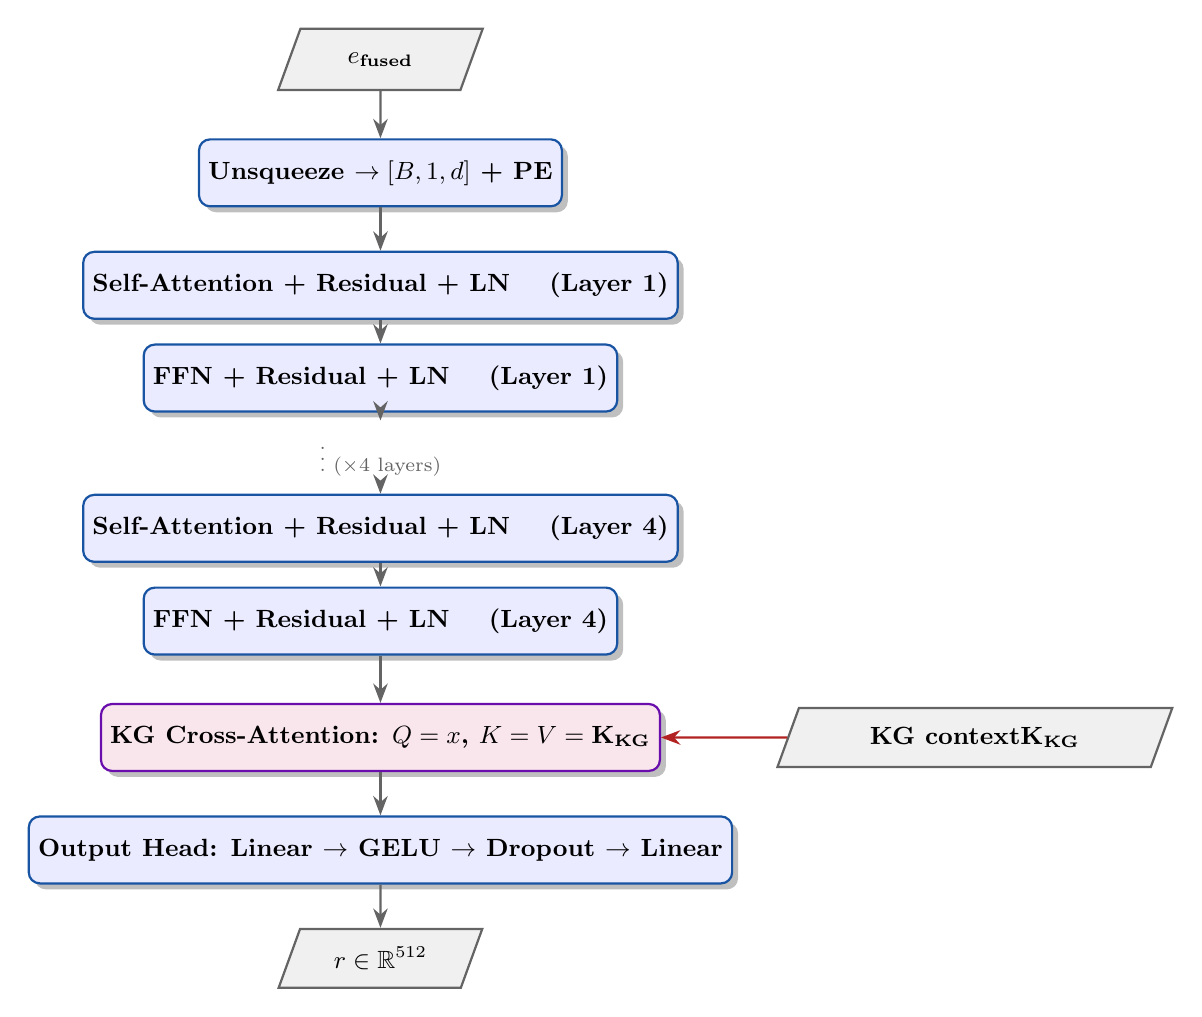
\begin{tikzpicture}[node distance=0.6cm, font=\small]
  \node[io] (ef2) {$e_\text{fused}$};
  \node[block, below=0.6cm of ef2]
    (uns) {Unsqueeze $\to [B,1,d]$ + PE};

  \node[block, below=0.55cm of uns, minimum width=5.5cm]
    (sa1) {Self-Attention + Residual + LN \quad (Layer 1)};
  \node[block, below=0.3cm of sa1, minimum width=5.5cm]
    (ff1) {FFN + Residual + LN \quad (Layer 1)};
  \node[mivagray, font=\scriptsize, below=0.1cm of ff1] (dots) {$\vdots$ (×4 layers)};
  \node[block, below=0.1cm of dots, minimum width=5.5cm]
    (saL) {Self-Attention + Residual + LN \quad (Layer 4)};
  \node[block, below=0.3cm of saL, minimum width=5.5cm]
    (ffL) {FFN + Residual + LN \quad (Layer 4)};

  \node[blockP, below=0.6cm of ffL, minimum width=5.5cm]
    (cross) {KG Cross-Attention: $Q=x$, $K=V=\mathbf{K}_\text{KG}$};
  \node[io, right=1.6cm of cross] (kgctx2) {KG context\\$\mathbf{K}_\text{KG}$};

  \node[block, below=0.55cm of cross, minimum width=5.5cm]
    (oh) {Output Head: Linear $\to$ GELU $\to$ Dropout $\to$ Linear};

  \node[io, below=0.55cm of oh] (r) {$r \in \R^{512}$};

  \draw[arrow] (ef2) -- (uns);
  \draw[arrow] (uns) -- (sa1);
  \draw[arrow] (sa1) -- (ff1);
  \draw[arrow] (ff1) -- (dots);
  \draw[arrow] (dots) -- (saL);
  \draw[arrow] (saL) -- (ffL);
  \draw[arrow] (ffL) -- (cross);
  \draw[arrowR] (kgctx2) -- (cross);
  \draw[arrow]  (cross) -- (oh);
  \draw[arrow]  (oh) -- (r);
\end{tikzpicture}
\caption{Transformer Reasoning Module architecture. KG cross-attention grounds the
output in structured medical knowledge.}
\label{fig:reason}
\end{figure}

\begin{plainbox}{In Plain English}
The Transformer Reasoning Module is the ``thinking'' part of the system.
After all information has been fused into one vector, the module re-reads it four
times (four encoder layers)---each pass refining its understanding, like a student
re-reading a dense paragraph.
After the self-attention passes, it opens the ``knowledge encyclopaedia'' (the KG
context) and asks: ``Does any of this factual knowledge about livers and tumours help
me answer the question better?'' The cross-attention mechanism is that consultation.
The result is an embedding that captures not just the question but also the relevant
world knowledge needed to answer it.
\end{plainbox}

% ════════════════════════════════════════════════════════════
\section{Grad-CAM Visual Explainability}
% ════════════════════════════════════════════════════════════

\subsection{Motivation}

In safety-critical domains, a model must be \emph{interpretable}: clinicians need to
know \emph{what regions of the image} drove the model's decision.
Grad-CAM~\cite{gradcam} produces a heatmap localising these regions.

\subsection{Mathematical Formulation}

\begin{definition}{Gradient Weights $\alpha_k^c$}{alphak}
Let $A^k \in \R^{H \times W}$ be the $k$-th feature map at the target convolutional
layer, and $y^c$ the score for class $c$ (before softmax). The importance weight is:
\[
  \alpha_k^c
  = \underbrace{\frac{1}{Z}\sum_{i=1}^H\sum_{j=1}^W}_{\text{global avg.\ pooling}}
    \frac{\partial y^c}{\partial A_{ij}^k}
\]
where $Z = H \times W$ is the spatial resolution.
\end{definition}

\begin{definition}{Grad-CAM Heatmap}{gcam}
\[
  L^c_{\text{Grad-CAM}}
  = \ReLU\!\left(\sum_k \alpha_k^c\, A^k\right)
\]
The $\ReLU$ retains only features with a \emph{positive} influence on class $c$.
The map is normalised to $[0,1]$ and upsampled to input resolution.
\end{definition}

\begin{theorem}{Class Discriminativity of Grad-CAM}{gcamdisc}
The Grad-CAM map $L^c_{\text{Grad-CAM}}$ is \emph{class-discriminative}:
if $\tilde{L}^{c}$ and $\tilde{L}^{c'}$ are normalised maps for classes $c \neq c'$,
then in general $\tilde{L}^{c} \neq \tilde{L}^{c'}$, because the gradient weights
$\alpha_k^c$ depend on $\partial y^c/\partial A_{ij}^k$, which differs per class.
\end{theorem}

\begin{algorithm}[H]
\caption{Grad-CAM Heatmap Generation}
\label{alg:gradcam}
\begin{algorithmic}[1]
\Require model $f$, input image $I$, target class $c$ (optional), target convolutional layer $\ell$
\Ensure Grad-CAM heatmap $\text{CAM} \in [0,1]^{H \times W}$
\State Register forward hook on $\ell$ to capture activations $A \in \R^{C \times H' \times W'}$
\State Register backward hook on $\ell$ to capture gradients $G$
\State $y \leftarrow f(I)$ \Comment{Forward pass}
\If{$c = \text{nil}$}
  \State $c \leftarrow \arg\max(y)$ \Comment{Use predicted class}
\EndIf
\State $f.\text{zero\_grad}()$
\State $y[0,c].\text{backward}()$ \Comment{Backward pass}
\State $\alpha_k \leftarrow \dfrac{1}{H'W'}\displaystyle\sum_{i,j} G[k,i,j]$  \Comment{Global average pool over spatial dims}
\State $\text{cam} \leftarrow \displaystyle\sum_k \alpha_k \cdot A[k,:,:]$
  \Comment{Weighted sum of activation maps}
\State $\text{cam} \leftarrow \ReLU(\text{cam})$
\State $\text{CAM} \leftarrow \text{cam} / (\max(\text{cam}) + \varepsilon)$
\State \Return $\text{CAM}$
\end{algorithmic}
\end{algorithm}

\begin{figure}[H]
\centering
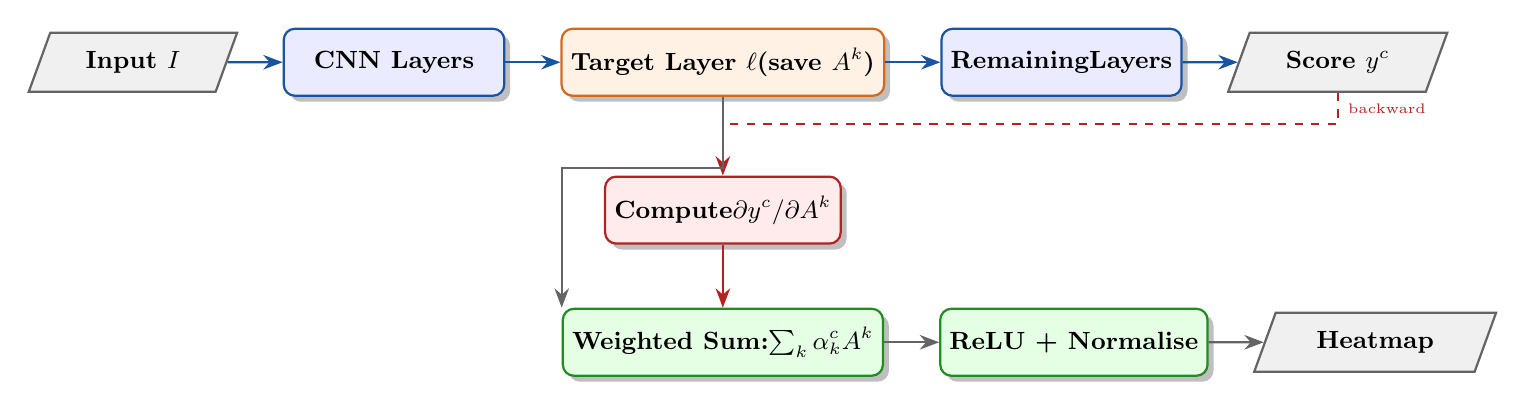
\begin{tikzpicture}[font=\small, node distance=0.6cm and 0.8cm]
  % Row 1: Forward
  \node[io] (inp) {Input $I$};
  \node[block, right=0.7cm of inp] (conv) {CNN Layers};
  \node[blockO, right=0.7cm of conv, minimum width=2.2cm]
    (tgt) {Target Layer $\ell$\\\small(save $A^k$)};
  \node[block, right=0.7cm of tgt] (rest) {Remaining\\Layers};
  \node[io, right=0.7cm of rest] (yc) {Score $y^c$};

  % Row 2: Backward
  \node[blockR, below=1.0cm of tgt, minimum width=2.2cm]
    (grad) {Compute\\$\partial y^c/\partial A^k$};

  % Row 3: CAM
  \node[blockG, below=0.8cm of grad, minimum width=3.5cm]
    (wsum) {Weighted Sum:\\$\sum_k \alpha_k^c A^k$};
  \node[blockG, right=0.7cm of wsum]
    (relu) {ReLU + Normalise};
  \node[io, right=0.7cm of relu] (heat) {Heatmap};

  \draw[arrowB] (inp)  -- (conv);
  \draw[arrowB] (conv) -- (tgt);
  \draw[arrowB] (tgt)  -- (rest);
  \draw[arrowB] (rest) -- (yc);
  \draw[arrowR, dashed] (yc.south) -- ++(0,-0.4)
        node[midway,right,font=\tiny]{backward}
        -| (grad.north);
  \draw[arrowR] (grad.south) -- (wsum.north);
  \draw[arrow]  (tgt.south)  -- ++(0,-0.3) -- ++(0,-0.6)
        -| (wsum.north west);
  \draw[arrow] (wsum)  -- (relu);
  \draw[arrow] (relu)  -- (heat);
\end{tikzpicture}
\caption{Grad-CAM computation flow. Activations and gradients are captured via
PyTorch hooks; the weighted combination produces the class-discriminative heatmap.}
\label{fig:gradcam}
\end{figure}

\begin{plainbox}{In Plain English}
Grad-CAM is like asking the AI: ``\emph{Show me where you were looking in this image
when you made your decision.}''
It works by running the image through the model (forward pass), getting the score for
the predicted disease, then tracing \emph{backwards} through the network to see which
neurons fired most strongly for that prediction, and specifically which image regions
activated those neurons.
The result is a colourful heatmap overlaid on the image: bright red/yellow means
``the model paid a lot of attention here'', while dark blue means ``irrelevant
region''. A good diagnostic AI should highlight the tumour, not the patient's name tag.
\end{plainbox}

% ════════════════════════════════════════════════════════════
\section{Complete MIVA-KNIGHT System}
% ════════════════════════════════════════════════════════════

\subsection{End-to-End Inference}

\begin{definition}{MIVA-KNIGHT Inference Function}{infer}
\[
  \hat{y},\;\text{CAM}
  = \text{MIVA-KNIGHT}(q,\, e_\text{img},\, e_\text{voice},\, e_\text{sensor},\,
    \mathcal{D},\, \kg)
\]
The six-step computational graph is:
\begin{align}
  &\text{Step 1:}\quad
    \mathcal{R} = \text{HybridRetrieve}(q, \mathcal{D}, \kg, \alpha)
    \label{step1}\\
  &\text{Step 2:}\quad
    e_\text{text} = \Enc(q), \quad
    e_m = \mathbf{0} \text{ if absent}
    \label{step2}\\
  &\text{Step 3:}\quad
    \efused, A = \text{Fusion}(e_\text{text},\, e_\text{img},\,
    e_\text{voice},\, e_\text{sensor})
    \label{step3}\\
  &\text{Step 4:}\quad
    \mathbf{K}_\text{KG} = \bigl[\Enc(\text{name}(e))\bigr]_{e \in \text{NER}(q)}
    \label{step4}\\
  &\text{Step 5:}\quad
    r,\, A_\text{KG} = \text{Reasoning}(\efused, \mathbf{K}_\text{KG})
    \label{step5}\\
  &\text{Step 6:}\quad
    \hat{y} = \FFN(r), \quad
    \text{CAM} = \text{GradCAM}(f_\theta, e_\text{img})
    \label{step6}
\end{align}
\end{definition}

\begin{algorithm}[H]
\caption{MIVA-KNIGHT End-to-End Inference}
\label{alg:e2e}
\begin{algorithmic}[1]
\Require query $q$; modality embeddings (optional); document corpus $\mathcal{D}$
\Ensure response $\hat{y}$, explanation dict
\State \textbf{--- Step 1: Hybrid Retrieval ---}
\State $\mathcal{R} \leftarrow \text{HybridRetrieve}(q, \mathcal{D}, \kg, \alpha=0.6)$
\State
\State \textbf{--- Step 2: Encode / pad modalities ---}
\If{$e_\text{text} = \text{nil}$}
  $e_\text{text} \leftarrow \Enc(q)$
\EndIf
\ForAll{$m \in \{\text{image, voice, sensor}\}$ with $e_m = \text{nil}$}
  \State $e_m \leftarrow \mathbf{0}_{d_m}$
\EndFor
\State
\State \textbf{--- Step 3: Multi-modal Fusion ---}
\State $\efused, A \leftarrow \text{Fusion}(e_\text{text}, e_\text{img}, e_\text{voice}, e_\text{sensor})$
\State
\State \textbf{--- Step 4: KG context ---}
\State $\mathcal{E} \leftarrow \text{NER}(q)$
\State $\mathbf{K}_\text{KG} \leftarrow
       [\Enc(\text{name}(e))]_{e \in \mathcal{E}}$
\State
\State \textbf{--- Step 5: Transformer Reasoning ---}
\State $r, A_\text{KG} \leftarrow \text{Reasoning}(\efused, \mathbf{K}_\text{KG})$
\State
\State \textbf{--- Step 6: Generate Response + Explainability ---}
\State $\hat{y} \leftarrow \text{ResponseHead}(r)$
\State $\text{CAM} \leftarrow \text{GradCAM}(f_\theta, e_\text{img})$
\State
\State \Return $\hat{y},\;\{\mathcal{R}, \mathcal{E}, \efused, A, r, A_\text{KG}, \text{CAM}\}$
\end{algorithmic}
\end{algorithm}

% ════════════════════════════════════════════════════════════
\section{Training Loss Functions}
% ════════════════════════════════════════════════════════════

\subsection{Multi-Objective Training}

\begin{definition}{MIVA-KNIGHT Total Loss}{totloss}
\[
  \boxed{\mathcal{L}_\text{total}
  = \mathcal{L}_\text{task}
  + \lambda_1 \mathcal{L}_\text{contrastive}
  + \lambda_2 \mathcal{L}_\text{KG}
  + \lambda_3 \mathcal{L}_\text{explain}}
\]
Default hyperparameters: $\lambda_1=1.0$, $\lambda_2=0.5$, $\lambda_3=0.3$.
\end{definition}

\begin{table}[H]
\centering
\caption{Loss function components.}
\begin{tabular}{lccp{5.5cm}}
\toprule
\textbf{Loss term} & \textbf{Symbol} & \textbf{$\lambda$} & \textbf{Purpose} \\
\midrule
Task (classification) & $\mathcal{L}_\text{task}$ & 1.0 &
  Correct label prediction \\
Contrastive (InfoNCE) & $\mathcal{L}_\text{contrastive}$ & 1.0 &
  Cross-modal embedding alignment \\
KG Consistency & $\mathcal{L}_\text{KG}$ & 0.5 &
  Embeddings respect KG structure \\
Explainability & $\mathcal{L}_\text{explain}$ & 0.3 &
  Interpretable attention distributions \\
\bottomrule
\end{tabular}
\end{table}

\subsection{Individual Loss Terms}

\subsubsection{Task Loss}

\begin{definition}{Cross-Entropy Task Loss}{celoss}
\[
  \mathcal{L}_\text{task}
  = -\sum_{c} y_c \log \hat{y}_c
  = \text{CrossEntropy}(\hat{y},\, y)
\]
\end{definition}

\subsubsection{KG Consistency Loss (TransE-Inspired)}

\begin{definition}{Margin Ranking KG Loss}{kgloss}
Inspired by TransE~\cite{transe}:
\[
  \mathcal{L}_\text{KG}
  = \sum_{(h,r,t)\in\kgE}
    \max\!\bigl(0,\;\gamma - f(h,r,t) + f(h',r,t')\bigr)
\]
where $f(h,r,t)$ scores a valid triple (high is good) and $f(h',r,t')$ scores a
corrupted triple (low is good); $\gamma > 0$ is the margin.
The simplified implementation uses:
\[
  \mathcal{L}_\text{KG}
  = \mathbb{E}\!\left[\max\!\bigl(0,\;
    \gamma - \|e_\text{text} - e_\text{KG}\|_2\bigr)\right]
\]
\end{definition}

\subsubsection{Explainability Loss}

\begin{definition}{Attention Regularisation Loss}{exploss}
\textbf{Unsupervised} (attention diversity):
\[
  \mathcal{L}_\text{explain}^{\text{unsup}} = -\text{Std}(A)
\]
\textbf{Supervised} (match human annotation $A^*$):
\[
  \mathcal{L}_\text{explain}^{\text{sup}} = \|A - A^*\|_2^2
\]
\end{definition}

\begin{algorithm}[H]
\caption{MIVA-KNIGHT Multi-Objective Training Step}
\label{alg:train}
\begin{algorithmic}[1]
\Require batch $\{(x_i, y_i)\}$; model $f_\theta$; loss weights $\lambda_1, \lambda_2, \lambda_3$; optimiser
\Ensure updated parameters $\theta$
\State $(\hat{y}, A, r, \ldots) \leftarrow f_\theta(x)$  \Comment{Forward pass}
\State $\mathcal{L}_\text{task} \leftarrow \text{CrossEntropy}(\hat{y}, y)$
\State $\mathcal{L}_\text{contr} \leftarrow \text{InfoNCE}(e_\text{text}, e_\text{img}, \tau=0.07)$
\State $\mathcal{L}_\text{KG} \leftarrow \max\!\bigl(0, \gamma - \|e_\text{text} - e_\text{KG}\|_2\bigr).\text{mean}()$
\State $\mathcal{L}_\text{exp} \leftarrow -\text{Std}(A)$
\State $\mathcal{L} \leftarrow \mathcal{L}_\text{task}
       + \lambda_1\mathcal{L}_\text{contr}
       + \lambda_2\mathcal{L}_\text{KG}
       + \lambda_3\mathcal{L}_\text{exp}$
\State $\mathcal{L}.\text{backward}()$  \Comment{Compute gradients}
\State $\theta \leftarrow \theta - \eta\,\nabla_\theta\mathcal{L}$  \Comment{Parameter update (Adam/SGD)}
\end{algorithmic}
\end{algorithm}

\begin{plainbox}{In Plain English}
Training MIVA-KNIGHT is like grading students on four separate report cards
simultaneously:
\begin{enumerate}
  \item \textbf{Task grade}: Did you get the right medical answer?
  \item \textbf{Cross-modal grade}: Do matching text--image pairs cluster together in
        the embedding space?
  \item \textbf{Knowledge grade}: Do your embeddings respect the facts in the medical
        knowledge graph (e.g.\ \emph{liver} near \emph{tumour})?
  \item \textbf{Interpretability grade}: Are your attention weights focused and
        explainable, rather than uniformly spread?
\end{enumerate}
The $\lambda$ weights say how much each grade matters: task and contrastive are most
important ($\lambda=1$), KG is moderately important ($\lambda=0.5$), and
interpretability is a soft regulariser ($\lambda=0.3$).
\end{plainbox}

% ════════════════════════════════════════════════════════════
\section{Evaluation Metrics}
% ════════════════════════════════════════════════════════════

\subsection{Classification Quality}

\begin{definition}{Accuracy}{acc}
\[
  \text{Accuracy} = \frac{|\{i : \hat{y}_i = y_i\}|}{N}
\]
Target: $\geq 90\%$.
\end{definition}

\begin{definition}{Macro F1 Score}{f1}
For class $c$:
\[
  \text{Precision}_c = \frac{\text{TP}_c}{\text{TP}_c + \text{FP}_c},\quad
  \text{Recall}_c = \frac{\text{TP}_c}{\text{TP}_c + \text{FN}_c}
\]
\[
  F1_c = \frac{2\cdot\text{Precision}_c\cdot\text{Recall}_c}
              {\text{Precision}_c + \text{Recall}_c},\quad
  F1_\text{macro} = \frac{1}{|C|}\sum_{c \in C} F1_c
\]
Macro-F1 weights all classes equally, which is crucial for imbalanced medical
datasets.
\end{definition}

\subsection{Retrieval Quality}

\begin{definition}{Mean Reciprocal Rank (MRR)}{mrr}
\[
  \text{MRR} = \frac{1}{|Q|}\sum_{i=1}^{|Q|} \frac{1}{r_i}
\]
where $r_i$ is the rank of the first relevant document for query $i$.
MRR $= 1.0$ means the relevant document is always ranked first.
\end{definition}

\begin{lemma}{MRR Bound}{mrrbound}
$0 \leq \text{MRR} \leq 1$.
The lower bound is achieved when no relevant document is ever retrieved;
the upper bound when the relevant document is always ranked first.
\end{lemma}

\subsection{Interpretability}

\begin{definition}{Normalised Attention Entropy}{attentropy}
\[
  H(A) = -\sum_i \hat{A}_i \log(\hat{A}_i + \varepsilon),\quad
  \hat{A} = \frac{A}{\sum A}
\]
\[
  \text{Interpretability} = 1 - \frac{H(A)}{H_{\max}},\quad
  H_{\max} = \log(|A|)
\]
Score $= 1.0$: maximally focused attention (one dominant region).
Score $= 0.0$: uniform attention (uninformative).
\end{definition}

\subsection{Latency}

\begin{definition}{Inference Latency Statistics}{lat}
Over $N_\text{runs}=100$ trials (after 10-run warm-up):
\[
  \mu = \mathbb{E}[t],\quad
  \sigma = \sqrt{\mathbb{E}[(t-\mu)^2]},\quad
  t_{50} = \text{Median}(t),\quad
  t_{95} = \text{Percentile}_{95}(t)
\]
Target: $\mu < 2$ seconds for real-time clinical use.
\end{definition}

\begin{table}[H]
\centering
\caption{Summary of all evaluation metrics.}
\begin{tabular}{llcc}
\toprule
\textbf{Metric} & \textbf{Formula} & \textbf{Range} & \textbf{Target} \\
\midrule
Accuracy     & $|\hat{y}=y|/N$         & $[0,1]$     & $\geq 0.90$ \\
Macro-F1     & $\text{avg}_c F1_c$      & $[0,1]$     & $\geq 0.88$ \\
MRR          & $\frac{1}{|Q|}\sum 1/r_i$& $[0,1]$     & $\geq 0.80$ \\
Interpretability& $1-H/H_\text{max}$   & $[0,1]$     & $\geq 0.60$ \\
Latency (mean)& $\mathbb{E}[t]$         & $[0,\infty)$& $<2$\,s \\
\bottomrule
\end{tabular}
\end{table}

% ════════════════════════════════════════════════════════════
\section{System Summary and Mathematical Recap}
% ════════════════════════════════════════════════════════════

\subsection{Complete Mathematical Formulation}

\begin{tcolorbox}[
  enhanced, breakable,
  colback=mivablue!4, colframe=mivablue,
  title={\bfseries\large MIVA-KNIGHT: Complete Mathematical Summary},
  fonttitle=\color{white},
  attach boxed title to top center={yshift=-3mm},
  boxed title style={colback=mivablue},
  arc=6pt
]
\textbf{Step 1 — Modality Encoding \& Projection:}
\[
  e_m = \Enc_m(x_m),\quad h_m = W_m e_m \in \R^{512}
\]

\textbf{Step 2 — Multi-Modal Fusion:}
\[
  \efused = \text{MeanPool}\!\Bigl(\LN\!\bigl[\mathbf{X}' + \FFN(\mathbf{X}')\bigr]\Bigr),
  \quad \mathbf{X}' = \LN\!\bigl(\mathbf{X} + \MHA(\mathbf{X})\bigr)
\]

\textbf{Step 3 — Contrastive Alignment:}
\[
  \mathcal{L}_\text{contr}
  = -\sum_i \log\frac{\exp(S_{ii})}{\sum_j \exp(S_{ij})},
  \quad S = \hat{E}_1\hat{E}_2^\top/\tau
\]

\textbf{Step 4 — Transformer Reasoning + KG Grounding:}
\[
  r = \text{OutputHead}\!\Bigl(x + \text{Attention}(x, \mathbf{K}_\text{KG},
  \mathbf{K}_\text{KG})\Bigr),\quad
  x = \text{TransformerEncoder}^{(4)}(\efused)
\]

\textbf{Step 5 — Response Generation:}
\[
  \hat{y} = \FFN(r), \quad
  \text{CAM}^c = \ReLU\!\left(\sum_k \alpha_k^c A^k\right)
\]

\textbf{Step 6 — Training Objective:}
\[
  \mathcal{L} = \mathcal{L}_\text{task}
  + \lambda_1\mathcal{L}_\text{contr}
  + \lambda_2\mathcal{L}_\text{KG}
  + \lambda_3\mathcal{L}_\text{explain}
\]
\end{tcolorbox}

\subsection{Component Interaction Diagram}

\begin{figure}[H]
\centering
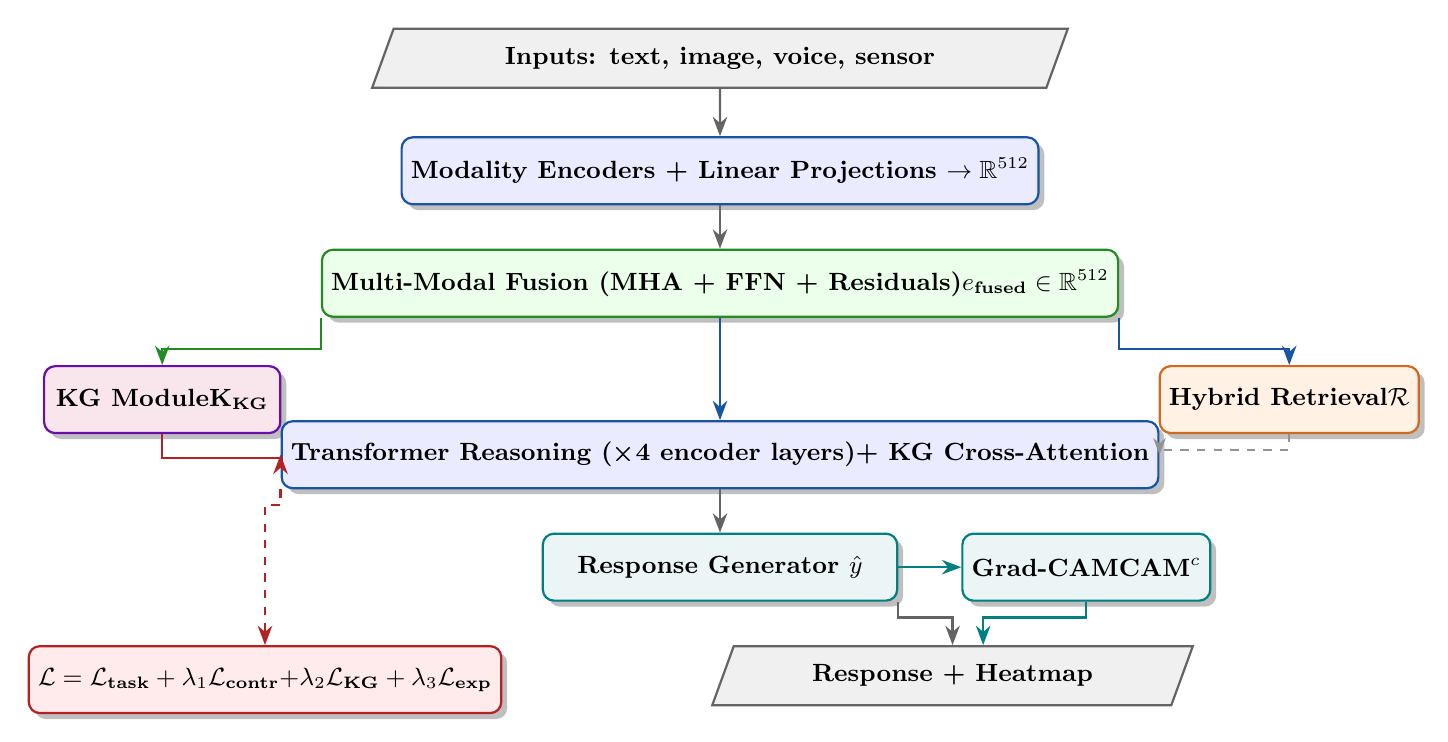
\begin{tikzpicture}[font=\small, node distance=0.55cm and 0.65cm]

\node[io, minimum width=6.5cm] (inputs)
  {Inputs: text, image, voice, sensor};

\node[block, below=0.6cm of inputs, minimum width=6.5cm]
  (enc) {Modality Encoders + Linear Projections $\to \R^{512}$};

\node[block, below=0.55cm of enc, minimum width=6.5cm,
      fill=green!8, draw=mivagreen]
  (fus) {Multi-Modal Fusion (MHA + FFN + Residuals)\\
         $\efused \in \R^{512}$};

\node[blockP, below left=0.6cm and 0.5cm of fus,
      minimum width=3.0cm]
  (kg3) {KG Module\\$\mathbf{K}_\text{KG}$};

\node[blockO, below right=0.6cm and 0.5cm of fus,
      minimum width=3.0cm]
  (ret) {Hybrid Retrieval\\$\mathcal{R}$};

\node[block, below=1.3cm of fus, minimum width=6.5cm]
  (reas) {Transformer Reasoning (×4 encoder layers)\\
          + KG Cross-Attention};

\node[block, below=0.55cm of reas, minimum width=4.5cm,
      fill=teal!8, draw=mivateal]
  (gen2) {Response Generator $\hat{y}$};

\node[blockT, right=0.8cm of gen2, minimum width=2.5cm]
  (gc2) {Grad-CAM\\$\text{CAM}^c$};

\node[blockR, below left=0.55cm and 0.5cm of gen2,
      minimum width=3.5cm]
  (loss2) {$\mathcal{L} = \mathcal{L}_\text{task}
            + \lambda_1\mathcal{L}_\text{contr}$\\
            $+ \lambda_2\mathcal{L}_\text{KG}
            + \lambda_3\mathcal{L}_\text{exp}$};

\node[io, below right=0.55cm and 0.3cm of gen2,
      minimum width=3.5cm]
  (out2) {Response + Heatmap};

\draw[arrow]  (inputs) -- (enc);
\draw[arrow]  (enc)    -- (fus);
\draw[arrowG] (fus.south west) -- ++(0,-0.4) -| (kg3.north);
\draw[arrowB] (fus.south east) -- ++(0,-0.4) -| (ret.north);
\draw[arrowB] (fus.south) -- ++(0,-1.0) -| (reas.north);
\draw[arrowR] (kg3.south) -- ++(0,-0.3) -| (reas.west);
\draw[dasharrow] (ret.south) -- ++(0,-0.2) -| (reas.east);
\draw[arrow]  (reas)   -- (gen2);
\draw[arrowT] (gen2)   -- (gc2);
\draw[arrowR,dashed] (reas.south west) -- ++(0,-0.2) -| (loss2.north);
\draw[arrow]  (gen2.south east) -- ++(0,-0.2) -| (out2.north);
\draw[arrowT] (gc2.south) -- ++(0,-0.2) -| (out2.north east);
\end{tikzpicture}
\caption{MIVA-KNIGHT component interaction diagram. Solid arrows: forward data flow.
Dashed arrows: training signal or auxiliary information flow.}
\label{fig:interact}
\end{figure}

% ════════════════════════════════════════════════════════════
\section{Implementation Notes and Next Steps}
% ════════════════════════════════════════════════════════════

\begin{table}[H]
\centering
\caption{Implemented components vs.\ production requirements.}
\begin{tabular}{lcc}
\toprule
\textbf{Component} & \textbf{Implemented} & \textbf{Production Notes} \\
\midrule
Knowledge Graph (in-memory)     & \checkmark & Connect to Neo4j \\
Hybrid RAG-LightRAG Retrieval   & \checkmark & Scale to millions of docs \\
Multi-modal Fusion Layer        & \checkmark & Add cross-modal contrastive pre-training \\
Contrastive Learning            & \checkmark & Use hard-negative mining \\
Transformer Reasoning (4-layer) & \checkmark & Scale to 12--24 layers \\
Grad-CAM Explainability         & \checkmark & Add SHAP / integrated gradients \\
Complete E2E Pipeline           & \checkmark & Wrap in FastAPI microservice \\
Multi-Objective Training Loss   & \checkmark & Add curriculum learning schedule \\
Evaluation Metrics              & \checkmark & Add BLEU/ROUGE for generation \\
Voice Processing                & $\circ$    & Integrate Whisper ASR + TTS \\
\bottomrule
\end{tabular}
\end{table}

\begin{plainbox}{Final Plain-English Summary}
MIVA-KNIGHT is built like a team of specialist analysts working together:
\begin{enumerate}
  \item \textbf{The Librarian} (Hybrid Retrieval) fetches the most relevant documents
        from both a semantic index and a medical reference book.
  \item \textbf{The Translators} (Modality Encoders \& Projections) convert text,
        images, audio, and sensor readings into a common vocabulary.
  \item \textbf{The Coordinator} (Multi-Modal Fusion) combines all translated inputs,
        deciding whose opinion matters most for this question.
  \item \textbf{The Expert} (Transformer Reasoning + KG) thinks deeply, consulting
        the encyclopaedia of medical facts to ground the answer.
  \item \textbf{The Communicator} (Response Generator) produces the final answer.
  \item \textbf{The Auditor} (Grad-CAM) points to exactly which evidence drove the
        conclusion, so a human expert can verify it.
\end{enumerate}
Training all six roles simultaneously—with four different ``report cards'' (losses)—
produces a system that is accurate, factually grounded, and interpretable.
\end{plainbox}

% ════════════════════════════════════════════════════════════
%  BIBLIOGRAPHY
% ════════════════════════════════════════════════════════════
\begin{thebibliography}{9}
\bibitem{gradcam}
  R.~R. Selvaraju et al.,
  ``Grad-CAM: Visual Explanations from Deep Networks via Gradient-Based
    Localization,''
  \emph{ICCV}, 2017.

\bibitem{transe}
  A.~Bordes et al.,
  ``Translating Embeddings for Modeling Multi-Relational Data,''
  \emph{NeurIPS}, 2013.

\bibitem{bert}
  J.~Devlin et al.,
  ``BERT: Pre-training of Deep Bidirectional Transformers for Language
    Understanding,''
  \emph{NAACL}, 2019.

\bibitem{infonce}
  A.~van den Oord et al.,
  ``Representation Learning with Contrastive Predictive Coding,''
  \emph{arXiv:1807.03748}, 2018.

\bibitem{transformer}
  A.~Vaswani et al.,
  ``Attention Is All You Need,''
  \emph{NeurIPS}, 2017.
\end{thebibliography}

\end{document}
